%% ID: trapdoor
%% TITLE: Trapdoor
%% TYPE: question
%% QUESTIONTYPE:  numerical
%% CONCEPTS: forces, moments, newtoni
%% VIDEOS: 
%% LEVEL: 3
%% TOPIC: mechanics/statics
%% ORDER: 8

\begin{problem}[AS1989AddPQ1p] %balancing moments
{\question{A uniform rectangular trap door of mass \vari{m} is hinged at one of its ends. It is held open making an angle \quantity{\theta}{60$^{\circ}$} to the horizontal with a force of magnitude \vari{F} at the open end acting perpendicular to the trap door. Find an expression for \vari{F} and find the value of \vari{\tan{\varphi}}, where \vari{\varphi} is the angle made by the line of action of the reaction force at the hinge above the horizontal.}
}
{\textit{Adapted with permission from UCLES, AS Level Additional Physics, June 1989, Paper 1, Question 1}}
{\answer{\valuedef{F}{\frac{1}{4}mg}{;} \valuedef{\tan{\varphi}}{\frac{7\sqrt{3}}{3}}{}}
\begin{figure}
	\centering
	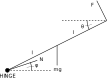
\includegraphics[width=0.4\textwidth]{Statics_trapdoor_hinge}
	\caption{}
	\label{fig:Statics_trapdoor_hinge}
\end{figure}
Figure \ref{fig:Statics_trapdoor_hinge} shows the trap door, where \vari{N} is the reaction force at the hinge. If the trap door has some length \vari{2l} then, taking moments about the hinge and noting that the trap door is in equilibrium, we find that
\begin{equation*}
2lF-lmg\cos(\theta)=0	
\end{equation*}
\begin{equation*}
F=\frac{1}{2}mg\cos(\theta)	
\end{equation*}

Replacing \vari{\theta} with its numerical value gives:
\begin{equation*}
F = \frac{1}{2}mg\cos{60}	
\end{equation*}
\begin{equation*}	
\Rightarrow F = \frac{1}{4}mg 	
\end{equation*}
	
Now we want to find the angle at which the force at the hinge acts and so we need to look at the equilibria in each direction at the hinge. Looking at the horizontal equilibrium at the hinge,
\begin{equation*}
N\cos(\varphi)-F\sin(\theta)=0	
\end{equation*}	
\begin{equation}
N\cos(\varphi)=F\sin(\theta)	 \label{eq:Statics_trapdoor_1}
\end{equation}	

And considering the vertical equilibrium at the hinge,
\begin{equation*}
N\sin(\varphi)+F\cos(\theta)-mg=0	
\end{equation*}
\begin{equation}
N\sin(\varphi)=mg-F\cos(\theta)	\label{eq:Statics_trapdoor_2}
\end{equation}

In order to find \vari{\varphi}, we divide equation \ref{eq:Statics_trapdoor_2} by equation \ref{eq:Statics_trapdoor_1} to get
\begin{equation*}
\tan(\varphi)=\frac{mg}{F\sin(\theta)}-\cot(\theta)	
\end{equation*}	
Using the numbers calculated earlier and those from the question:
\begin{equation*}
\tan(\varphi)=\frac{mg}{\frac{1}{4}mg\sin(60^\circ)}-\cot(60^\circ)	
\end{equation*}	
\begin{equation*}
\tan(\varphi)=\frac{8}{\sqrt{3}}-\frac{1}{\sqrt{3}}=\frac{7}{\sqrt{3}}	
\end{equation*}	
\begin{equation*} 
\Rightarrow \tan{\varphi} = \frac{7\sqrt{3}}{3}	
\end{equation*}
}
\end{problem}